\chapter{Clustering}


\section{Similarity and dissimilarity}

\begin{description}
    \item[Similarity] \marginnote{Similarity}
        Measures how alike two objects are.
        Often defined in the range $[0, 1]$.

    \item[Dissimilarity] \marginnote{Dissimilarity}
        Measures how two objects differ.
        0 indicates no difference while the upper-bound varies.
\end{description}

\begin{table}[ht]
    \centering
    \renewcommand{\arraystretch}{2}
    \begin{tabular}{c | c | c}
        \textbf{Attribute type} & \textbf{Dissimilarity} & \textbf{Similarity} \\
        \hline
        Nominal & $d(p, q) = \begin{cases} 0 & \text{if } p=q \\ 1 & \text{if } p \neq q \end{cases}$ & $s(p, q) = 1 - d(p, q)$ \\
        \hline
        Ordinal & $d(p, q) = \frac{\vert p - q \vert}{V}$ with $p, q \in \{ 0, \dots, V \}$ & $s(p, q) = 1 - d(p, q)$ \\
        \hline
        Interval or ratio & $d(p, q) = \vert p - q \vert$ & $s(p, q) = \frac{1}{1 + d(p, q)}$
    \end{tabular}
    \caption{Similarity and dissimilarity by attribute type}
\end{table}

\begin{description}
    \item[Similarity properties] \phantom{}
        \begin{enumerate}
            \item $\texttt{sim}(p, q) = 1$ iff $p = q$. 
            \item $\texttt{sim}(p, q) = \texttt{sim}(q, p)$. 
        \end{enumerate}
\end{description}


\subsection{Distance}

Given two $D$-dimensional data entries $p$ and $q$, possible distance metrics are:
\begin{descriptionlist}
    \item[Minkowski distance ($L_r$)] \marginnote{Minkowski distance}
        \[ \texttt{dist}(p, q) = \left( \sum_{d=1}^{D} \vert p_d - q_d \vert^r \right)^{\frac{1}{r}} \]
        where $r$ is a parameter.

        Common values for $r$ are:
        \begin{descriptionlist}
            \item[$r = 1$] 
                Corresponds to the $L_1$ norm.
                It is useful for discriminating 0 distance and near-0 distance as 
                an $\varepsilon$ change in the data corresponds to an $\varepsilon$ change in the distance.
            \item[$r = 2$]
                Corresponds to the Euclidean distance or $L_2$ norm.
            \item[$r = \infty$]
                Corresponds to the $L_\infty$ norm.
                Considers only the dimensions with the maximum difference.
        \end{descriptionlist}
    
    \item[Mahalanobis distance] \marginnote{Mahalanobis distance}
        \[ \texttt{dist}(p, q) = \sqrt{ (p-q) \matr{\Sigma}^{-1} (p-q)^T } \]
        where $\matr{\Sigma}$ is the covariance matrix of the dataset.
        The Mahalanobis distance of $p$ and $q$ increases when the segment connecting them 
        points towards a direction of greater variation of the data.

        \begin{figure}[h]
            \centering
            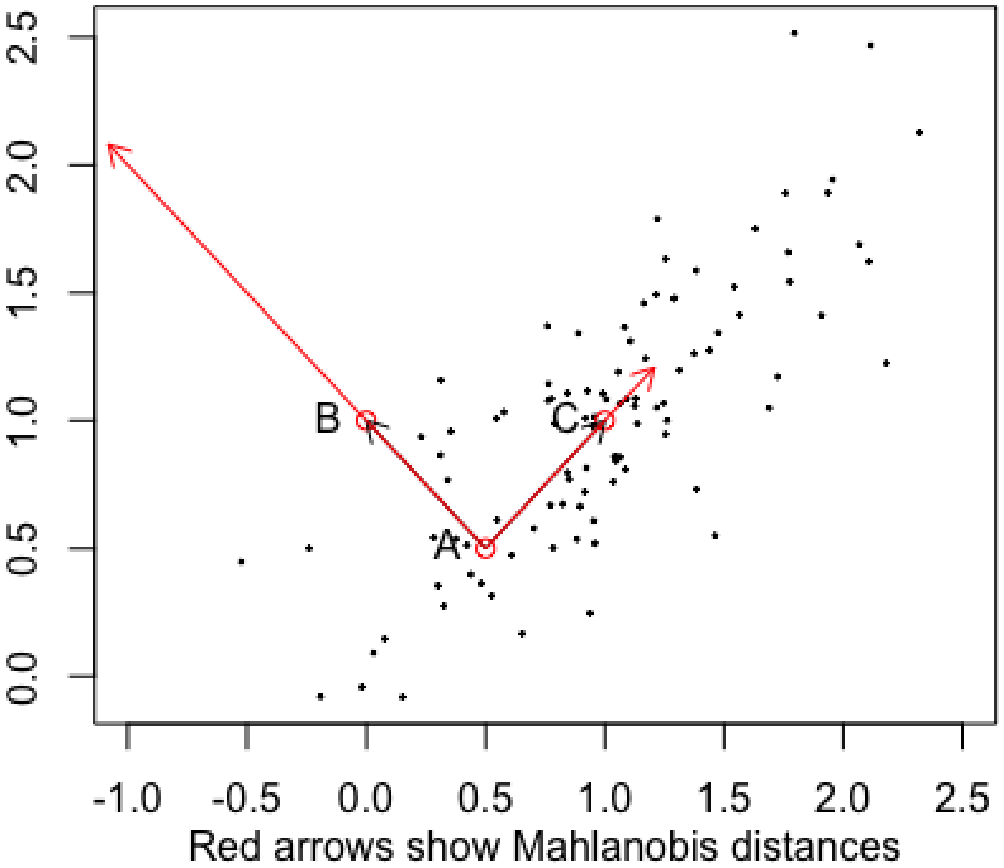
\includegraphics[width=0.35\textwidth]{img/mahalanobis.png}
            \caption{The Mahalanobis distance between $(A, B)$ is greater than $(A, C)$, while the Euclidean distance is the same.}
        \end{figure}
\end{descriptionlist}

\subsubsection{Distance properties}
\begin{descriptionlist}
    \item[Positive definiteness] 
        $\texttt{dist}(p, q) \geq 0$ and $\texttt{dist}(p, q) = 0$ iff $p = q$.
    \item[Symmetry] 
        $\texttt{dist}(p, q) = \texttt{dist}(q, p)$
    \item[Triangle inequality] 
        $\texttt{dist}(p, q) \leq \texttt{dist}(p, r) + \texttt{dist}(r, q)$
\end{descriptionlist}



\subsection{Vector similarity}

\begin{description}
    \item[Binary vectors]
        Given two examples $p$ and $q$ with binary features, we can compute the following values:
        \[ 
            \begin{split}
                M_{00} &= \text{ number of features that equals to 0 for both $p$ and $q$} \\
                M_{01} &= \text{ number of features that equals to 0 for $p$ and 1 for $q$} \\
                M_{10} &= \text{ number of features that equals to 1 for $p$ and 0 for $q$} \\
                M_{11} &= \text{ number of features that equals to 1 for both $p$ and $q$}
            \end{split}    
        \]
        Possible distance metrics are:
        \begin{descriptionlist}
            \item[Simple matching coefficient] \marginnote{Simple matching coefficient}
                $\texttt{SMC}(p, q) = \frac{M_{00} + M_{11}}{M_{00} + M_{01} + M_{10} + M_{11}}$ 
            \item[Jaccard coefficient] \marginnote{Jaccard coefficient}
                $\texttt{JC}(p, q) = \frac{M_{11}}{M_{01} + M_{10} + M_{11}}$ 
        \end{descriptionlist}

    \item[Cosine similarity] \marginnote{Cosine similarity}
        Cosine of the angle between two vectors:
        \[ \texttt{cos}(p, q) = \frac{p \cdot q}{\Vert p \Vert \cdot \Vert q \Vert} \]

    \item[Extended Jaccard coefficient (Tanimoto)] \marginnote{Extended Jaccard coefficient (Tanimoto)}
        Variation of the Jaccard coefficient for continuous values:
        \[ \texttt{T}(p, q) = \frac{p \cdot q}{\Vert p \Vert^2 + \Vert q \Vert^2 - p \cdot q} \]
\end{description}


\subsection{Correlation}

\begin{description}
    \item[Pearson's correlation] \marginnote{Pearson's correlation}
        Measure of linear relationship between a pair of quantitative attributes $e_1$ and $e_2$.
        To compute the Pearson's correlation, the values of $e_1$ and $e_2$ are first standardized and then ordered to obtain the vectors $\vec{e}_1$ and $\vec{e}_2$.
        The correlation is then computed as the dot product between $\vec{e}_1$ and $\vec{e}_2$:
        \[ \texttt{corr}(e_1, e_2) = \langle \vec{e}_1, \vec{e}_2 \rangle \]

        Pearson's correlation has the following properties:
        \begin{itemize}
            \item If the variables are independent, then the correlation is 0 (but not vice versa).
            \item If the correlation is 0, then there is no linear relationship between the variables.
            \item $+1$ implies positive linear relationship, $-1$ implies negative linear relationship.
        \end{itemize}

    \item[Symmetric uncertainty]
        Measure of correlation for nominal attributes:
        \[ U(e_1, e_2) = 2 \frac{H(e_1) + H(e_2) - H(e_1, e_2)}{H(e_1) + H(e_2)} \in [0, 1] \]
        where $H$ is the entropy.
\end{description}